\documentclass[]{article}
\usepackage[english]{babel}
\usepackage[utf8]{inputenc}
\usepackage{pdfpages}
\usepackage{amsthm}
\usepackage{amsfonts}
\usepackage{mathrsfs}
\usepackage{amssymb}
\usepackage{amsmath}
\usepackage[]{algorithm2e}


\usepackage{hyperref}
\hypersetup{
	colorlinks=true,
	breaklinks=true,
	linkcolor=blue,
	urlcolor=blue}
\newtheorem{thdef}{Definition}
\theoremstyle{remark}
\newtheorem{rk}{Remark}
\newtheorem{proposition}{Proposition}
\newtheorem{corollary}{Corollary}
\newcommand{\thref}[2]{\hyperref[#2]{#1 \ref*{#2}}}
\numberwithin{equation}{subsection}

\usepackage{url}
\usepackage[]{xcolor}
\definecolor{light-gray}{gray}{0.6}
\definecolor{blue}{RGB}{0,0,153}
\definecolor{blue1}{RGB}{0,102,204}
\definecolor{blue2}{RGB}{51,153,255}
\definecolor{blue3}{RGB}{0,153,153}
\definecolor{blue4}{RGB}{102,102,255}
\definecolor{red1}{RGB}{255,0,0}
\definecolor{orange1}{RGB}{255,153,51}
\definecolor{green}{RGB}{0,204,0}
\definecolor{purple}{RGB}{204,0,204}
\usepackage{graphicx}
\usepackage{multirow}
\usepackage{boxedminipage}
\usepackage{tikz}
\usetikzlibrary{calc} 

\setcounter{MaxMatrixCols}{20}

\tikzset{
  x=1ex,y=1ex,
  hwblock/.style={draw, rectangle, rounded corners=.3, very thick, fill=black!5, font=\sf, minimum height=5ex},
  hwbus/.style={very thick,>=stealth},
  hwwire/.style={thin, >=stealth, },
  hwword/.style={draw, rectangle, minimum height=3ex},
  bitwidth/.style={font=\scriptsize,midway,right}
}

\newcommand{\msbout}{m_{\text{out}}}
\newcommand{\appr}[1]{\widetilde{#1}}
\newcommand{\abserr}{\varepsilon}
\newcommand{\epssopc}{\abserr_{\text{r}}}
\newcommand{\epsfinalround}{\abserr_{\text{f}}}
\newcommand{\TODO}{\textbf{TODO}}
\newcommand{\y}{y}
\newcommand{\yM}{\boldsymbol{\y}}
\newcommand{\yout}{{y_{out}}}
\newcommand{\youtM}{\boldsymbol{\yout}}
\newcommand{\ys}{{y^*}}
\newcommand{\ysM}{\boldsymbol{\ys}}
%\newcommand{\dy}{{\delta_{y}}}
%\newcommand{\dy}{{E_{y}}}
%\newcommand{\dy}{{\mathcal{E}_{y}}}
%\newcommand{\dy}{{\mathscr{E}_{y}}}
%\newcommand{\dy}{{\mathfrak{E}_{y}}}
\newcommand{\dy}{{e_{y}}}
\newcommand{\dyM}{\boldsymbol{\dy}}
\newcommand{\ly}{{l_{\yout}}}
\newcommand{\lys}{\boldsymbol{l_{\ys}}}
\newcommand{\lx}{{l_x}}
\newcommand{\lt}{{l_t}}
\newcommand{\lu}{{l_u}}
\newcommand{\lyM}{\boldsymbol{\ly}}
\newcommand{\lysM}{\boldsymbol{\lys}}
\newcommand{\lxM}{\boldsymbol{\lx}}
\newcommand{\ltM}{\boldsymbol{\lt}}
\newcommand{\luM}{\boldsymbol{\lu}}
\newcommand{\wcpg}{\|\mathcal{H}_{\varepsilon}\|}
\newcommand{\tf}{\mathcal{H}}
\newcommand{\tfe}{\mathcal{H}_{\varepsilon}}
\newcommand{\errVt}{\boldsymbol{\varepsilon_t}}
\newcommand{\errVx}{\boldsymbol{\varepsilon_x}}
\newcommand{\errVy}{\boldsymbol{\varepsilon_{\ys}}}
\newcommand{\errV}{\boldsymbol{\varepsilon}}
\newcommand{\errVe}{\begin{pmatrix} \errVt \\ \errVx \\ \errVy \end{pmatrix}}
\newcommand{\efr}{{\varepsilon_{fr}}}
\newcommand{\efrM}{\boldsymbol{\efr}}



\title{Error Analysis}
\author{\\ \Large Antoine Martinet \\ \\\\\\\\\\\\\\ \\ \\ Master 2 Internship Report \\ \\ \\ \LARGE at CITI lab \\ INRIA's SOCRATE Team \\\\\\\\\\\\\\\\ \normalsize under the supervision of\\ \\ \Large Florent de Dinechin \\ \\ \\}
\date{2 February - 31 Jully, \\ \vspace{5pt} 2015}

\begin{document}
	\section{Notations}
		What is given by the user is:

		$\lyM$, the least significant bits desired for all outputs y\\

		$\luM$, the least significant bits desired for all inputs u\\

	What we want is the error $\dyM$ introduced by the whole filter, given all intermediates errors, in order to compute back those errors:

		$$\dyM < \frac{1}{2} \lyM$$
	
	Intermediate errors are defined as follows:

		$\errVy$, the error introduced computing y from t, x, and u\\
			
        $\errVx$, the error introduced computing x from t, x, and u\\

        $\errVt$, the error introduced computing t from t, x, and u\\

	What we search are:

		$\ltM$, the least significant bits desired for all intermediate variables t\\

		$\lxM$, the least significant bits desired for all state variables x\\
		
		\begin{figure}[h] 
		  \centering
		  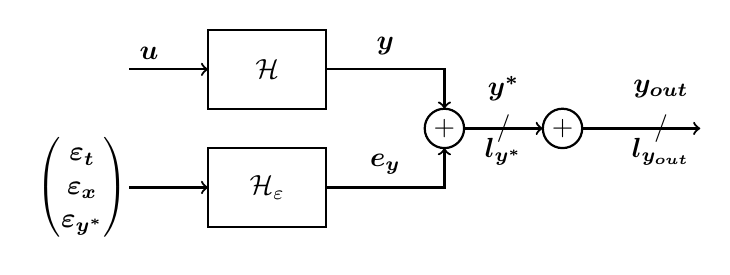
\begin{tikzpicture}[x=1cm,y=1cm]
			\draw (-2,0.5) rectangle ++(1.5,1)[thick] node [midway]{$\mathcal{H}$}; 
			\draw (-3, 1) -- (-2,1) [->, thick] node [above,near start]{$\boldsymbol{u}$}; 
			\draw (-0.5, 1)  -- (1,1) -- (1,0.5) [->, thick] node[xshift=-0.75cm,yshift=0.8cm]{$\yM$}; 

			\draw (-2,-1) rectangle ++(1.5,1)[thick] node [midway]{$\mathcal{H}_{\abserr}$}; 
			\draw (-3, -0.5) -- (-2,-0.5) [->, thick] node[xshift=-1.6cm, yshift=0.0cm]{$\errVe$};
			\draw (2.5,0.25)  circle (0.25)[thick] node []{+}; 
			\draw (-0.5, -0.5) -- (1,-0.5) -- (1,0) [->, thick] node [xshift=-0.75cm,yshift=-0.2cm]{$\dyM$}; 

			\draw (1,0.25) circle (0.25) [thick] node {$+$}; 
			\draw (1.25,0.25) -- (2.25,0.25)[->, thick] node [xshift=-0.5cm, yshift=0.5cm] {$\ysM$} node [xshift=-0.5cm, yshift=0cm] {/} node [xshift=-0.5cm, yshift=-0.3cm] {$\lysM$};
			\draw (2.75,0.25) -- (4.25,0.25)[->, thick] node [xshift=-0.5cm, yshift=0.5cm] {$\youtM$} node [xshift=-0.5cm, yshift=0cm] {/} node [xshift=-0.5cm, yshift=-0.3cm] {$\lyM$};
		  \end{tikzpicture}

		\caption{A signal view of the error propagation with respect to the ideal filter \label{fig:ltierror}}
		\end{figure}

		Further definitions:
		
		$$ \lysM = log_2 \lfloor \errVy \rfloor$$
		$$ \lxM  = log_2 \lfloor \errVx \rfloor$$
		$$ \ltM  = log_2 \lfloor \errVt \rfloor$$

	\section{Error Analysis}
	What Lopez claims:

	$$\dy = \wcpg \cdot \errVe$$
	
	Resuming, we want:

		$$\dyM < \frac{1}{2} \ly$$

		$$\Leftrightarrow$$

		$$\frac{1}{2} \ly > \wcpg \cdot \errVe$$

		$$\Leftrightarrow$$

		$$\frac{1}{2} \ly_i > \sum_{j=1}^n \wcpg_{i,j} \cdot \errV_j, \hspace{10pt} \forall 1 \leq i \leq n_y$$
	Idea: find the solution using PNL, trying to maximize the lsbs, so the error, respecting the previous constraint set:

		$$\sum \errV_i$$

\end{document}

